\subsection{Zonificación}
\label{subsec:cap4-zonificacion}
Cada entorno puede contar con factores que lo hagan más o menos apto para el desarrollo,
mortalidad, alimentación, dispersión, y reproducción de individuos. En esta sección, con el fin de
simplificar ciertos aspectos muy específicos que se encuentran fuera del alcance de este trabajo,
realizaremos ciertas hipótesis generales, justificadas para este caso de aplicación, pero puede
requerir una revisión en caso general. Estas hipótesis son, los valores observados en un
conjunto de puntos de control, pertenecientes a una zona, permiten la caracterización de dicha
zona como más o menos apta para desarrollo, mortalidad, alimentación, dispersión, y reproducción de
individuos. También consideramos que el tamaño de la zona, y por ende la cantidad de puntos de
control que pertenecen a ella, influye en la caracterización de las zonas.

La zonificación surge ante necesidad de dividir el espacio de estudio de una forma más granular,
para identificar a los individuos que pertenecen a zonas aptas y los que no. Los puntos de control
distribuidos en un área de estudio permiten estimar los niveles de riesgo e infestación
correspondiente a la abundancia de larvas por litro observadas.

Para determinar el tipo de zona de un individuo $m_{i}$ ubicado en $(x,y)$, primero se estima la
densidad relativa de larvas, para $m_{i}(x,y)$, utilizando interpolación espacial y posteriormente
se la clasifica utilizando una escala. Si consideramos a $u(x,y)$ el valor interpolado para
$m_{i}(x,y)$, entonces la densidad relativa de larvas de $m_{i}(x,y)$ es igual a $u(x,y)$. La
cantidad de larvas observadas en los puntos de control, pertenecientes a la zona de $m_{i}(x,y)$,
corresponden a los valores conocidos utilizados para la interpolación espacial, donde el tamaño de
la zona de $m(x,y)$ se encuentra determinado por $r$, que representa el radio una circunferencia
que tiene como centro a $(x,y)$. El tamaño de $r$, es un parámetro ajustable del modelo, mientras
más grande sea el tamaño de $r$, más puntos de control serán considerados para el cálculo de
$u(x,y)$. Por ejemplo en la \figref{fig:cap4-zonficiacion} podemos observar que existen 8 puntos
de control, cuyos valores son conocidos y se encuentran representados por
$[u_{1}, u_{2}, \dots ,u_{8}]$, de los cuales para estimar el valor de $u(x,y)$ con un radio de
tamaño igual a $r$, solo serán considerados $[u_{1}, u_{2},\dots,u_{5}]$.

\begin{figure}[!hptb]
\centering
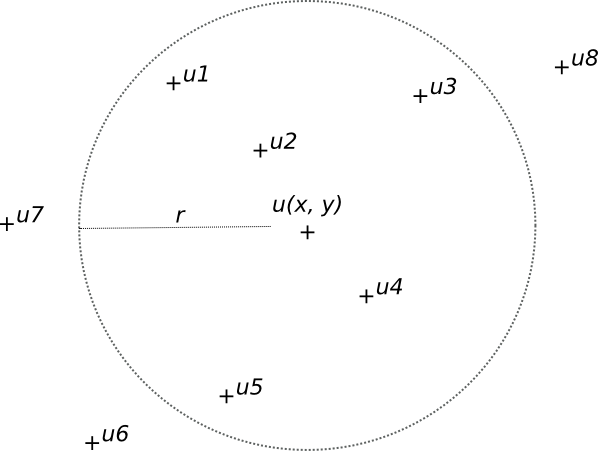
\includegraphics[width=0.6\textwidth]{capitulo-4/graphics/zonificacion.png}
\caption{\label{fig:cap4-zonficiacion} Relación entre el radio $r$, el valor de $u(x,y)$ a estimar y los valores conocidos.}
\end{figure}

El valor estimado de $u(x,y)$ es utilizado para clasificar la zona como \textit{Pésima},
\textit{Mala}, \textit{Regular}, \textit{Buena} u \textit{Óptima} con influencia positiva el
desarrollo, alimentación, dispersión, y reproducción de individuos y negativamente para la
mortalidad. Con la finalidad de utilizar un mismo criterio de clasificación para todos los
individuos, se define una escala única para este caso de estudio. Los valores de dicha escala son
agrupados por la capacidad de generar hembras adultas que eventualmente puedan llegar a oviponer.

Considerando que $u(x,y)$ representa densidad de relativa de larvas y que la escala a utilizar
para su clasificación se basa en su etapa adulta, se debe realizar una transición de los estados
larva a pupa y de pupa a adulto. Esta transición entre estados es necesaria para poder estimar la
cantidad de hembras adultas con capacidad reproductiva. Para realizar los cálculos
correspondientes hay que tener en cuenta las siguientes consideraciones :

\begin{itemize}
    \item Solo el $50$ \% de las larvas observadas son hembras \cite{otero2006stochastic, manrique1998desarrollo}.
    \item La temperatura media anual es de 25 \textcelsius \cite{website:mspbsHistoria2014}.
    \item La tasa mortalidad diaria natural de las larvas y pupas bajo optimas condiciones, a 25 \textcelsius, es igual a $0,01056$ 1/días, según las ecuaciones \eqref{eq:mortalidad-natural-larvas} y \eqref{eq:mortalidad-natural-pupas} respectivamente.
    \item La tasa de desarrollo, a 25 \textcelsius, de la larva hasta su emergencia a adulto es de $11,57$ días \cite{rueda1990temperature}.
    \item El $32,10$ \% de las hembras adultas no oviponen \cite{osoriopontificia}.
\end{itemize}

Estas consideraciones ayudan a simplificar la simulación de la transición de estados pasando de
larva a pupa y de pupa a adulto, con el fin de construir la escala de clasificación. Los valores
de cantidad de hembras con capacidad de oviponer, finalmente obtenidas a partir de $u(x,y)$ son
calculados para un entorno óptimo.


\begin{table}[!hptb]
    \begin{minipage}{\textwidth}
\begin{center}
    \caption{\label{tab:cap4-puntaje-zona} Escala de clasificación de las zonas de acuerdo a la densidad relativa de larvas.}
    \begin{tabular}{p{3cm} c c c c}
        \\
                     & Mínimo$^a$ & Máximo$^a$ & Hembras     & Hembras$^c$ \\
        Tipo de zona & $u(x,y)$   & $u(x,y)$   & Adultas$^b$ & Reproductivas$^c$ \\
        \hline
        \hline\\
        Pésima  & 0  & 19 & 8  & 5 \\
        Mala    & 20 & 35 & 15 & 10\\
        Regular & 36 & 51 & 22 & 15\\
        Buena   & 52 & 69 & 30 & 20\\
        Óptima  & 70 & --$^d$ & --$^d$ & --$^d$\\
    \end{tabular}
    \footnotetext[1]{Rango mínimo y máximo de $u(x,y)$ permitido para el tipo de zona.}
    \footnotetext[2]{Cantidad máxima de hembras adultas, al final del periodo de desarrollo.}
    \footnotetext[3]{Cantidad de hembras adultas con capacidad de oviponer.}
    \footnotetext[4]{No se estableció un límite superior para las zonas óptimas. }
\end{center}
    \end{minipage}
\end{table}

En la \tabref{tab:cap4-puntaje-zona} se pueden observar los rangos definidos para cada tipo de
zona, en donde $u$ es la densidad relativa de larvas en las coordenadas $(x,y)$. Los límites para
las zonas fueron determinados clasificando los valores, de las hembras reproductivas en, grupos
múltiplos de cinco. No se estableció un límite superior para las zonas óptimas debido a que los
valores mayores a el mínimo establecido, 70 larvas por litro, pertenecen a la misma categoría.
